%
% $Id$
%
% Describe important points about DODS servers.

\documentclass{article}
\usepackage{epsfig}
\usepackage{rotating}
% \usepackage{subfigure}
% \usepackage{vcode}
\usepackage{xspace}
% \usepackage{gloss}

% Change paragraph typesetting; eliminate indenting and add more space between
% paragraphs. 2/15/2000 jhrg
\setlength{\parindent}{0em}     % Amount of indentation
\addtolength{\parskip}{1ex}     % Vertical separation

% Sample macros including a URL which can be hyphenated. 
\newcommand{\httpd}{\texttt{httpd}\xspace}
\newcommand{\Cpp}{\rm {\small C}\raise.5ex\hbox{\footnotesize ++}\xspace}
\newcommand{\dap}{\rm {\small DAP}\raise.5ex\hbox{\footnotesize ++}\xspace}
\newcommand{\maewesturl}{http://maewest.gso.uri.edu/\-cgi-bin/\-nph-dsp/\-htn\_sst\_decloud/\-1992/\-i92098065016.htn\_d.Z\xspace}

\begin{document}

\title{Internet Server Architecture}
\author{James Gallagher\thanks{jgallagher@gso.uri.edu}
  \and Dan Holloway\thanks{d.holloway@gso.uri.edu}}
\date{\today \\ $Revision$ }

\maketitle
\tableofcontents

\section{Server Strategy}
\label{sec:strategy}

Three goals of DODS drive the data server's requirements. Thos goals are:
\begin{itemize}
\item Make remote data easy to access.

\item Do not presuppose how data will be used.

\item Provide a suite of data servers that are very easy to install and
  configure.
\end{itemize}

Data access:
\begin{itemize}
\item Provide web-standard access to data (HTML, ASCII). Simple clients such
  as web browsers and spreadsheets.

\item Provide access using representations specific to our software. Support
  complex analysis tools.
\end{itemize}

Flexible data use outlook:
\begin{itemize}
\item Metadata: Provide an easy way for people to add metadata to an existing
  dataset.
  
\item Allow for datasets which have very little metadata (nothing beyond a
  datatype such as \texttt{byte x[512][512]}).
\end{itemize}

Installation and configuration of the servers:
\begin{itemize}
\item Use \httpd. All the usual reasons: Of-the-shelf software, security,
  standard IPC, \ldots
  
\item Use CGI: Ease of installation, modularity. (But CGI is not without
  faults; security, sluggish performance, \ldots We're looking at ways to
  provide our server software in both CGI- and daemon-based configurations.)
\end{itemize}

\section{URLs Reference data}
\label{sec:URLs}

\begin{itemize}
\item In the DODS DAP, datasets are referenced using URLs. 

\item Each Dataset has a unique URL.

\item Each variable within a dataset cn be referenced independently using a
constraint expression appended to a URL.

\item Variables also maybe subsampled (providing a way for clients to ask for
  ony a small part of a single variable) using a constraint expressions.
\end{itemize}

\emph{[The following was copied from a SDD describing changes planned to our
  servers.  See DODS-doc/archive/design/server-arch/dods-server-sdd.tex.
  jhrg]}

Figure~\ref{fig:httpd-directories} shows an example \httpd configuration.
There are three \httpd configuration parameters that are shown in the
example.  The \texttt{DocumentRoot} parameter holds the root pathname of the
\httpd's document tree. The document root in the figure contains
subdirectories named \texttt{data/nc}, \texttt{data/hdf} and \texttt{data/ff}
that each holds data files (there's nothing special about these names;
any valid pathname will work).  The \texttt{ScriptAlias} parameter holds a
pathname where \httpd may find CGI programs.

For example, suppose that in the \texttt{data/nc} directory there is a data
file named \texttt{fnoc1.nc} and that the DODS server dispatch CGI is named
\texttt{nph-nc}.  For completeness, suppose that the domain name of the host
running the server configured as shown in Figure~\ref{fig:httpd-directories}
is \texttt{dcz.dods.org}. The DODS URL for this dataset would be
\begin{equation}
\texttt{http://dcz.dods.org/cgi-bin/nph-nc/data/nc/fnoc1.nc}
\label{url:simple}
\end{equation}
URL~\ref{url:simple} will return an error when typed into a web
browser\footnote{NB: This URL \emph{will} work when passed to a DODS client
  program but that's because those programs know they are dealing with a DODS
  URL and know how to append the various suffixes to get different responses.
  A web browser knows nothing about DODS so the user must append the
  suffix.}, however, because the server has not been asked to return any
result. Thus, the server returns a response which explains that the request
was an error, explains why and tells how to form a valid request.

A DODS server can return three different types of objects unique to DODS and
four responses that can be used by many different programs, including web
browsers. Each of the different responses are requested by appending a suffix
to the $<path>$ component of the DODS URL. The suffixes and the response they
generate are:
\begin{description}
\item[.das] Return the DODS DAS object, encoded as ASCII text.
\item[.dds] Return the DODS DDS object, encoded as ASCII text.
\item[.dods] Return the DODS DataDDS object, encoded in a multipart MIME
  document. 
\item[.asc] Return data in a CSV format which can be read by spreadsheet
  programs.
\item[.html] Return an HTML form which automatically builds a constraint
  expression that describes which data in the data source to access.
\item[.info] Return an HTML document which combines the metadata and
  ancillary data stored with the data source in a way that is easy(ier) to
  read than the text representation of the DAS and DDS objects.
\item[/] This suffix is unlike all the others in that it is added to the
  end of a directory name, \emph{not} a data source name. When the $<path>$
  part of a DODS URL ends in a slash (\texttt{/}) the server returns a
  listing of the named directory.
\end{description}
Thus to request HTML encoded metadata about the FNOC dataset shown in
URL~\ref{url:simple} you would append the suffix \texttt{.info} to the URL

\begin{equation}
\texttt{http://dcz.dods.org/cgi-bin/nph-nc/data/nc/fnoc1.nc.\textbf{info}}
\label{url:info}
\end{equation}

Accessing data from a DODS server usually involves more than simply appending
the suffix \texttt{.dods} or \texttt{.asc} to a URL. That is because most of
the time a data source holds far more information than the user (either human
or computer) wants or needs. DODS uses constraint expressions to describe the
parts of a data source that are desired. For example, suppose a particular
data file contains five variables, but a user wants only two of those
variables. A constraint expression can be used to request that only those two
variables be included in the server's response to the request for data. A
constraint expression is supplied using the Query String part of a URL. Even
though the syntax of the constraint expression language is fairly simple,
describing it is outside the scope of this paper. The syntax is fully
described in the DODS User's Guide. However, here are
two example URLs with constraints
\begin{equation}
\texttt{http://dcz.dods.org/cgi-bin/nph-nc/data/nc/fnoc1.nc.dods?u,v}
\label{url:ce1}
\end{equation}
\begin{equation}
\texttt{http://dcz.dods.org/} \cdots \texttt{/fnoc1.nc.dods?u[0:5][0][0:2:10]}
\label{url:ce2}
\end{equation}
URL~\ref{url:ce1} requests that data contained in just the variables $u$ and
$v$ be included in the response. URL~\ref{url:ce2} stipulates that only $u$
be returned and further limits the parts of the three dimensional
array\footnote{How did I know it was a three dimensional array? Look at the
  output of the DDS or Info responses from the server.} to the first six
rows, only column $0$ and the six planes numbered $0, 2, 4, \cdots, 10$.

\begin{figure}[h]
\begin{center}
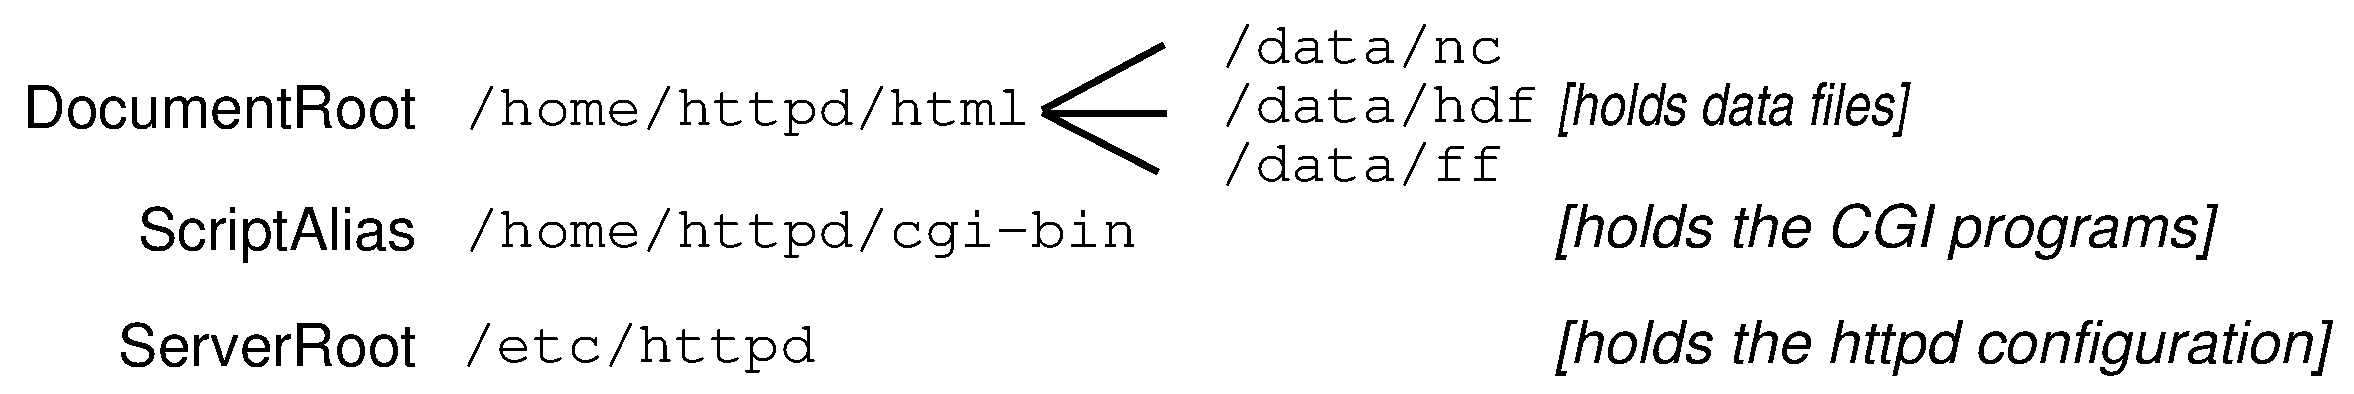
\epsfig{file=httpd-directories.eps,width=4.5in}
\caption{A typical directory structure for an Apache \texttt{httpd}
  installation (this is the installation found on RedHat Linux; other Unix
  installations might use different directories, but the essential
  organization is the same). Note that the directories \texttt{data/nc},
  \texttt{data/hdf} and \texttt{data/ff} are examples. The actual collection
  of directories, their names and contents have no more restrictions than any
  other directory on a Unix computer.}
\label{fig:httpd-directories}
\end{center}
\end{figure}

\section{Servers for Multifile Datasets}
\label{sec:multifile}

Definition: Multifile datasets are (essentially) relational datasets where
one or more variables are stored in separate files split by time, location,
\textit{et cetera}. For example, URI has a dataset which holds satellite
imagery.  Each file holds a single image and there are approximately 25,000
files, one for each pass of the satellite (about two per day).

\begin{itemize}
\item To the DODS software a dataset with many files is actually a collection
  of many datasets. 
  
\item DODS represents multifile datasets by creating a new dataset which
  describes the aggregation of the separate files (datasets to the DODS
  software). This dataset can be accessed by a regular DODS server. We often
  use the FreeForm server for this purpose (and call it a \emph{file server}
  in this special case). The FreeForm server has been modified to provide
  access to dates and times using a mechanism that can map a collection's
  \textit{ad hoc} scheme to a standard representation.
  
\item The dataset served by a file server typically lists URLs and dates
  (although a URL, or set of URLs, and other values that vary over those URLs
  could be contained in a file server's dataset).
  
\item Clients make a request to the file server asking for the URLs that
  span, for example, a range of dates.  They get back a list of URLs which
  can be used to access data that falls within that date range.
  
\item Since each URL is itself a complete dataset, it is possible that each
  one contains different variables with their own unique metadata. Often,
  however, the variables which can be accessed by any of the URLs returned by
  a file server are exactly the same type and only their capture time (for
  example) differs.
  
\item Clients must handle access access to a file server specially. They must
  know that to access `real' data a second dereference must take place.
  
\item We plan to build a server which can automatically perform the second
  dereference (which will encapsulate the actual organization of the
  dataset).
\end{itemize}

\section{Host Configuration}
\label{sec:configuration}

See Figure~\ref{fig:deployment}~(page~\pageref{fig:deployment}).

\begin{itemize}
\item A Machine can easily host several different DODS servers, one for each
  type of data it holds. Components common to all servers (see
  Section~\ref{sec:components}) are not duplicated.
  
\item A web daemon provides networking infrastructure, including security and
  logging.
  
\item Data are typically stored in files, but the actual storage form is not
  set by DODS. Some datasets are stored in RDBM systems, some in collections
  of files and some in a single file.
  
\item Our servers built using the \Cpp class library (called the \dap
  library) currently only run on UNIX, although they could run on Win32 in
  principle (the \dap library has been ported to Win32). Our Java-based
  servers run on both UNIX and Win32.\footnote{The Java-based servers use
    servlets instead of CGI and only support the basic objects in the DAP at
    this time.}
\end{itemize}

\begin{sidewaysfigure}[h]
\begin{center}
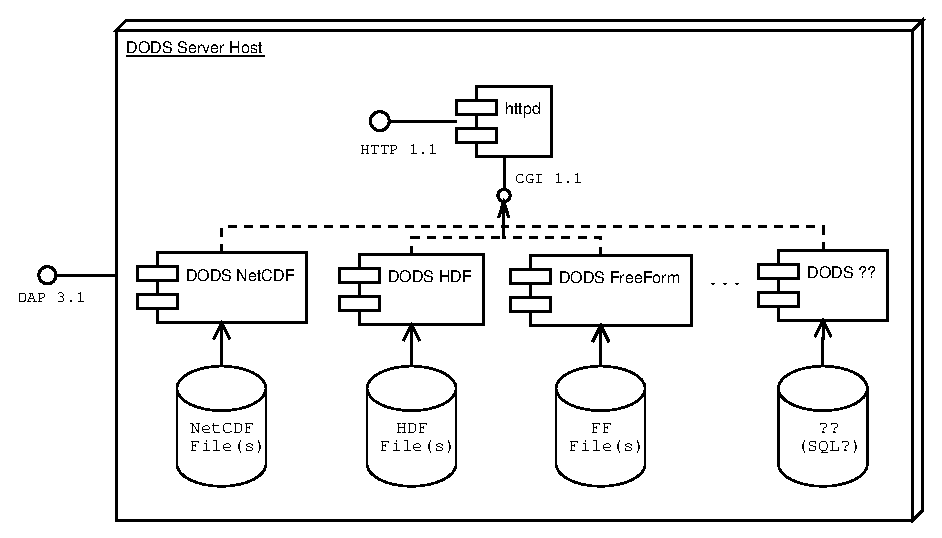
\epsfig{file=current-deployment.eps,width=7.5in}
\caption{A machine which hosts a DODS server must also have a web daemon
  running and provide access to the data served.}
\label{fig:deployment}
\end{center}
\end{sidewaysfigure}

\section{Components of a Server}
\label{sec:components}

See Figure~\ref{fig:dods-server-components}~(page~\pageref{fig:dods-server-components}).

\begin{itemize}
\item Most DODS servers for which we (DODS/URI) provide software are built
  using eight components, each of which is a separate program.

\item Each component of our server is written in either C++ or Perl. 
  
\item Each server has a dispatch component written in Perl. This handles
  parsing information from the request (separating the URL into the
  \texttt{pathname} and \texttt{query string} parts) and reading information
  from various environment variables.
  
\item Each server \emph{must} have three handlers for the three responses
  which define the DAP. These are the DAS, DDS and DataDDS.
  
\item Each server \emph{should} provide components which return other
  information:
\begin{itemize}
\item Data in ASCII
\item Information from the DAS and DDS combined and represented in
HTML
\item A \emph{very} simple interface to the dataset which can run in a web
browser (currently implemented in HTML and JavaScript)
\item A directory listing in HTML\footnote{See Section~\ref{sec:URLs}}
\end{itemize}
\end{itemize}

\begin{quote}
N.B.: Both the NetCDF and the FreeForm servers provide good examples of an
implementation of the components which generate DAS, DDS and DataDDS objects.
Look in the DODS/src/tools directory for the source code to the ASCII and
HTML response generators. The Perl code for the directory and dispatch
component can be found in DODS/etc.
\end{quote}

\begin{sidewaysfigure}[h]
\begin{center}
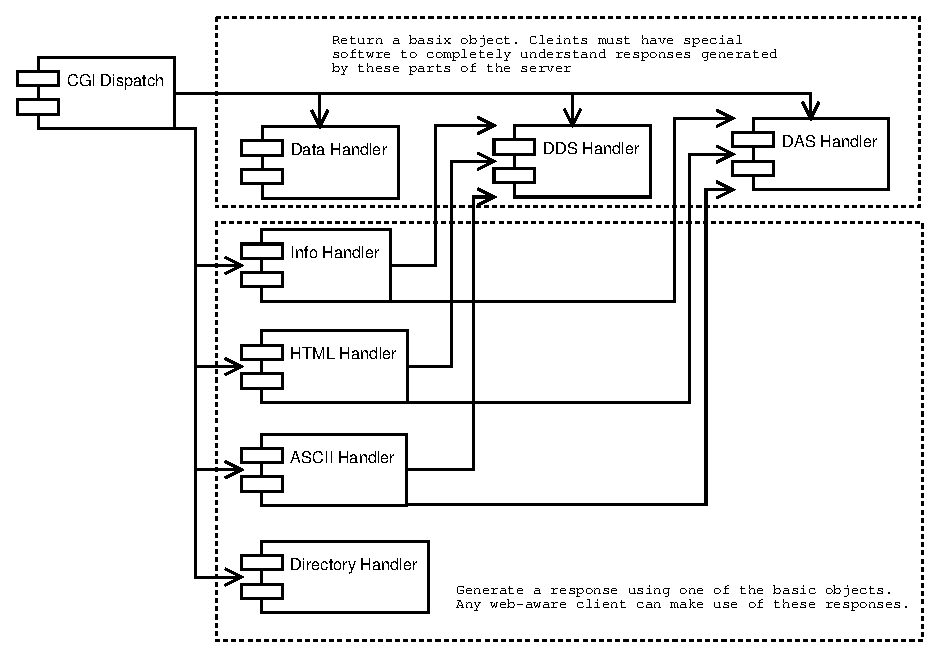
\epsfig{file=current-server-arch.eps,width=7.5in}
\caption{DODS servers are composed of eight components: the dispatch script,
  three components that return objects which form the core of the DAP and
  other components which return HTML or ASCII responses.}
\label{fig:dods-server-components}
\end{center}
\end{sidewaysfigure}

% \clearpage
% \appendix

% \section{ChangeLog}
% \begin{verbatim}

% $Log: internet-server-arch.tex,v $
% Revision 1.3  2000/11/06 19:57:13  jimg
% *** empty log message ***
%
% Revision 1.2  2000/11/06 18:43:11  jimg
% Fixed grammar & spelling errors.
%
% Revision 1.1  2000/11/06 18:41:02  jimg
% First version.
%

% \end{verbatim}

\end{document}
